\chapter{Event Selection}
\label{chap:Selection}

We require events to contain exactly three selected leptons. Events with different lepton compositions are further categorized into different channels: $eee$, $\mu\mu\mu$, $e\mu l$. In all three channels, the sum of the charges of three leptons are required to be 1 or -1. The leading leptons in all selected events are required to be matched with trigger objects via $\Delta R<$0.2. Within each channel, different regions are defined to further understand signal and background.

e$\mu\ell$ is the channel where the presence of the signal is expected. We require at least one pair of leptons of Opposite-Sign-Opposite-Flavor (OSOF). Such a requirement is achieved if:

\begin{itemize}
\item Both positively charged and negatively charged leptons are present.
\item Both electrons and muons are present.
\end{itemize}

Events with the presence of the same flavor leptons are categorized into $eee$ or $\mu\mu\mu$ channels to study the background composition. 
%%%%%%%%%%%%%%%%%%%%%%%%%%%%%%%%%%%%%%%%%%%%%%%%%%%%%%%%%%%%%
%%%%%%%%%%%%%%%%%%%%%%%%%%%%%%%%%%%%%%%%%%%%%%%%%%%%%%%%%%%%%
\section{Signal Region}
\label{sec:SR}

In $e\mu l$ channel, we set up our signal region (SR) targeting LFV signal processes. Apart from the OSOF pair, we require the events to have big MET (MET $>$ 20 GeV). Events with an Opposite-Sign-Same-Flavor (OSSF) lepton pair, the invariant mass of which is between 50 GeV and 106 GeV, are removed to suppress contribution from Z production. To further suppress background contribution, we require at least one jet and at most one b-tag jet.

Distributions of leading lepton $p_{T}$ and invariant mass of Opposite-Sign $e\mu$ pair are shown in Figure \ref{fig:SR}. Please note: Although we intend to deploy a data-driven technique to estimate non-prompt background in the actual analysis, all backgrounds in Figure \ref{fig:SR} are estimated using MC simulation only. This serves as a preliminary check to understand the components of different backgrounds in SR. 
\begin{figure}[tbh!]
 \begin{center}
 \begin{tabular}{cc}
 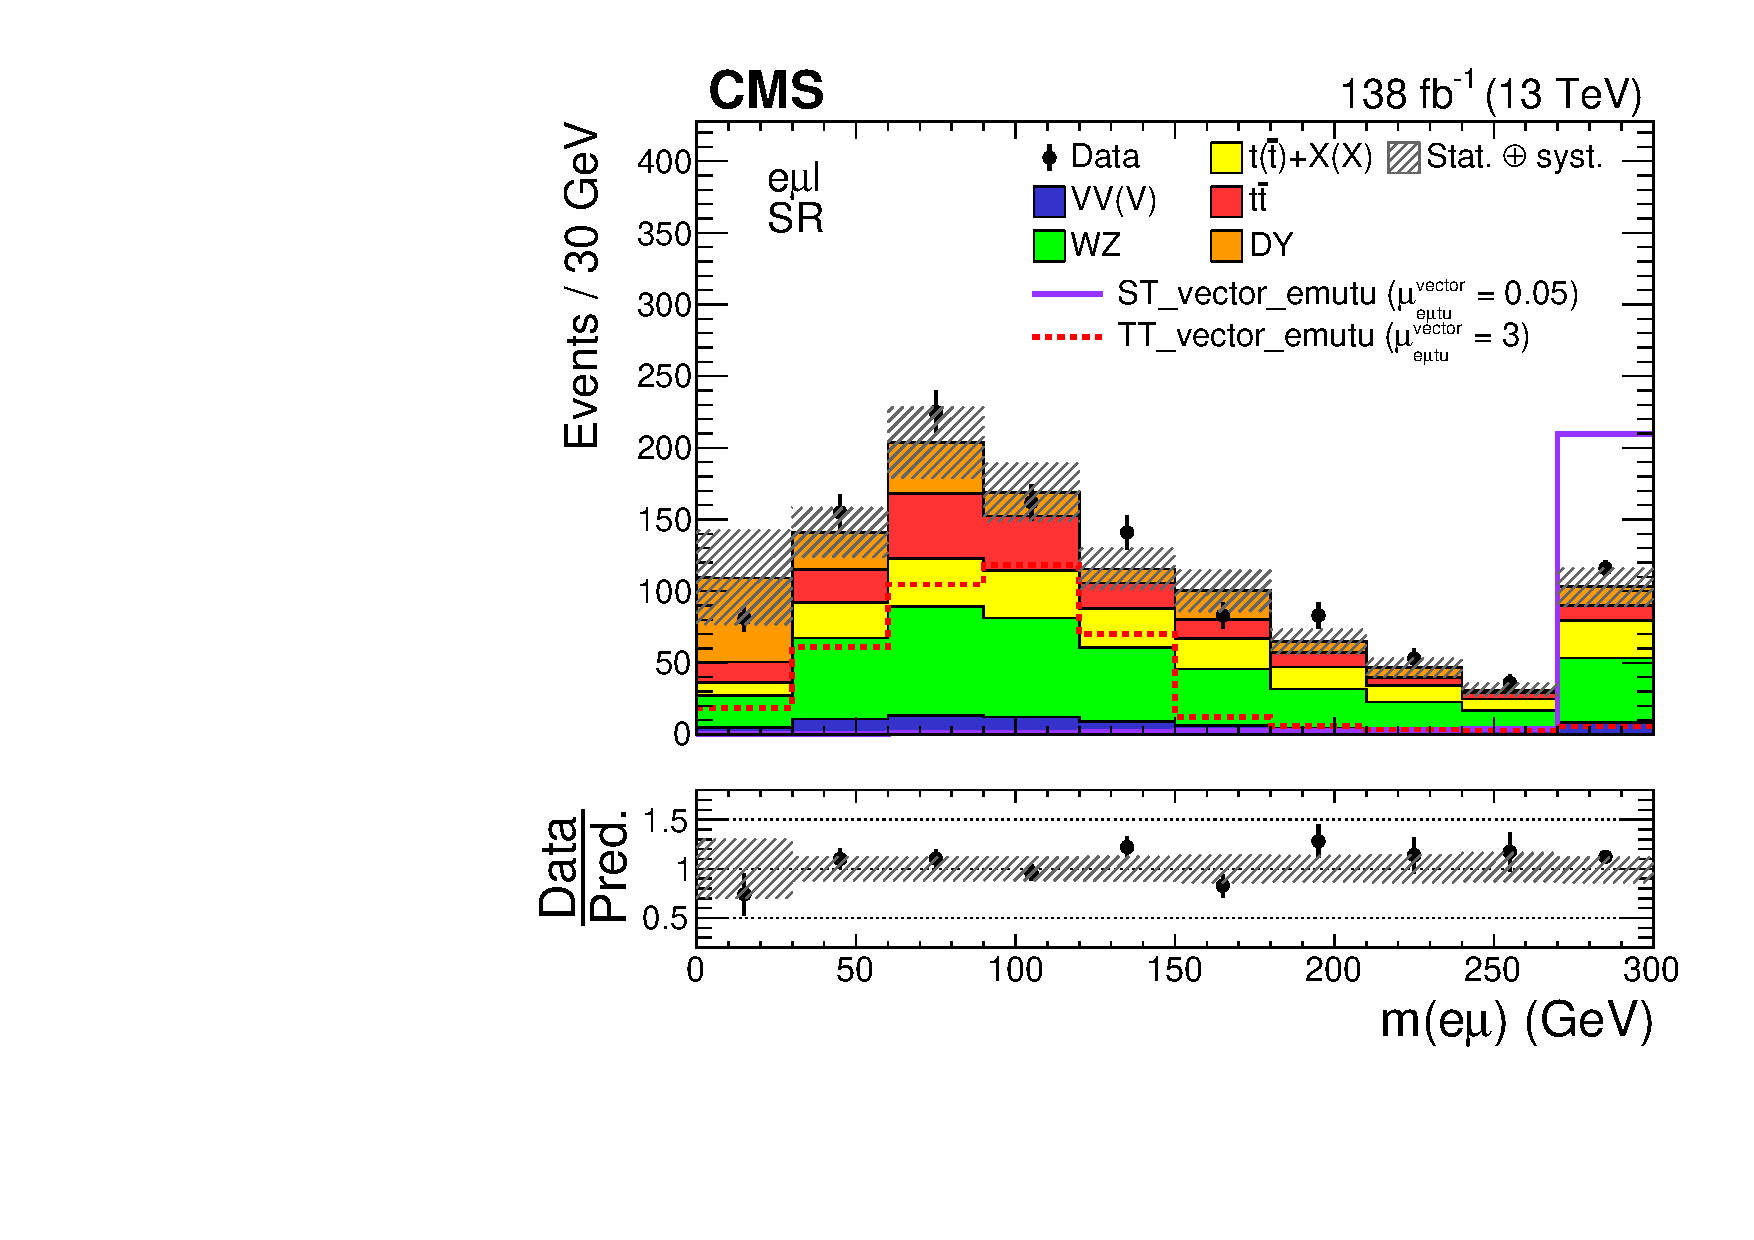
\includegraphics[width=0.45\textwidth]{figures/Part3/Selection/Memu}&
 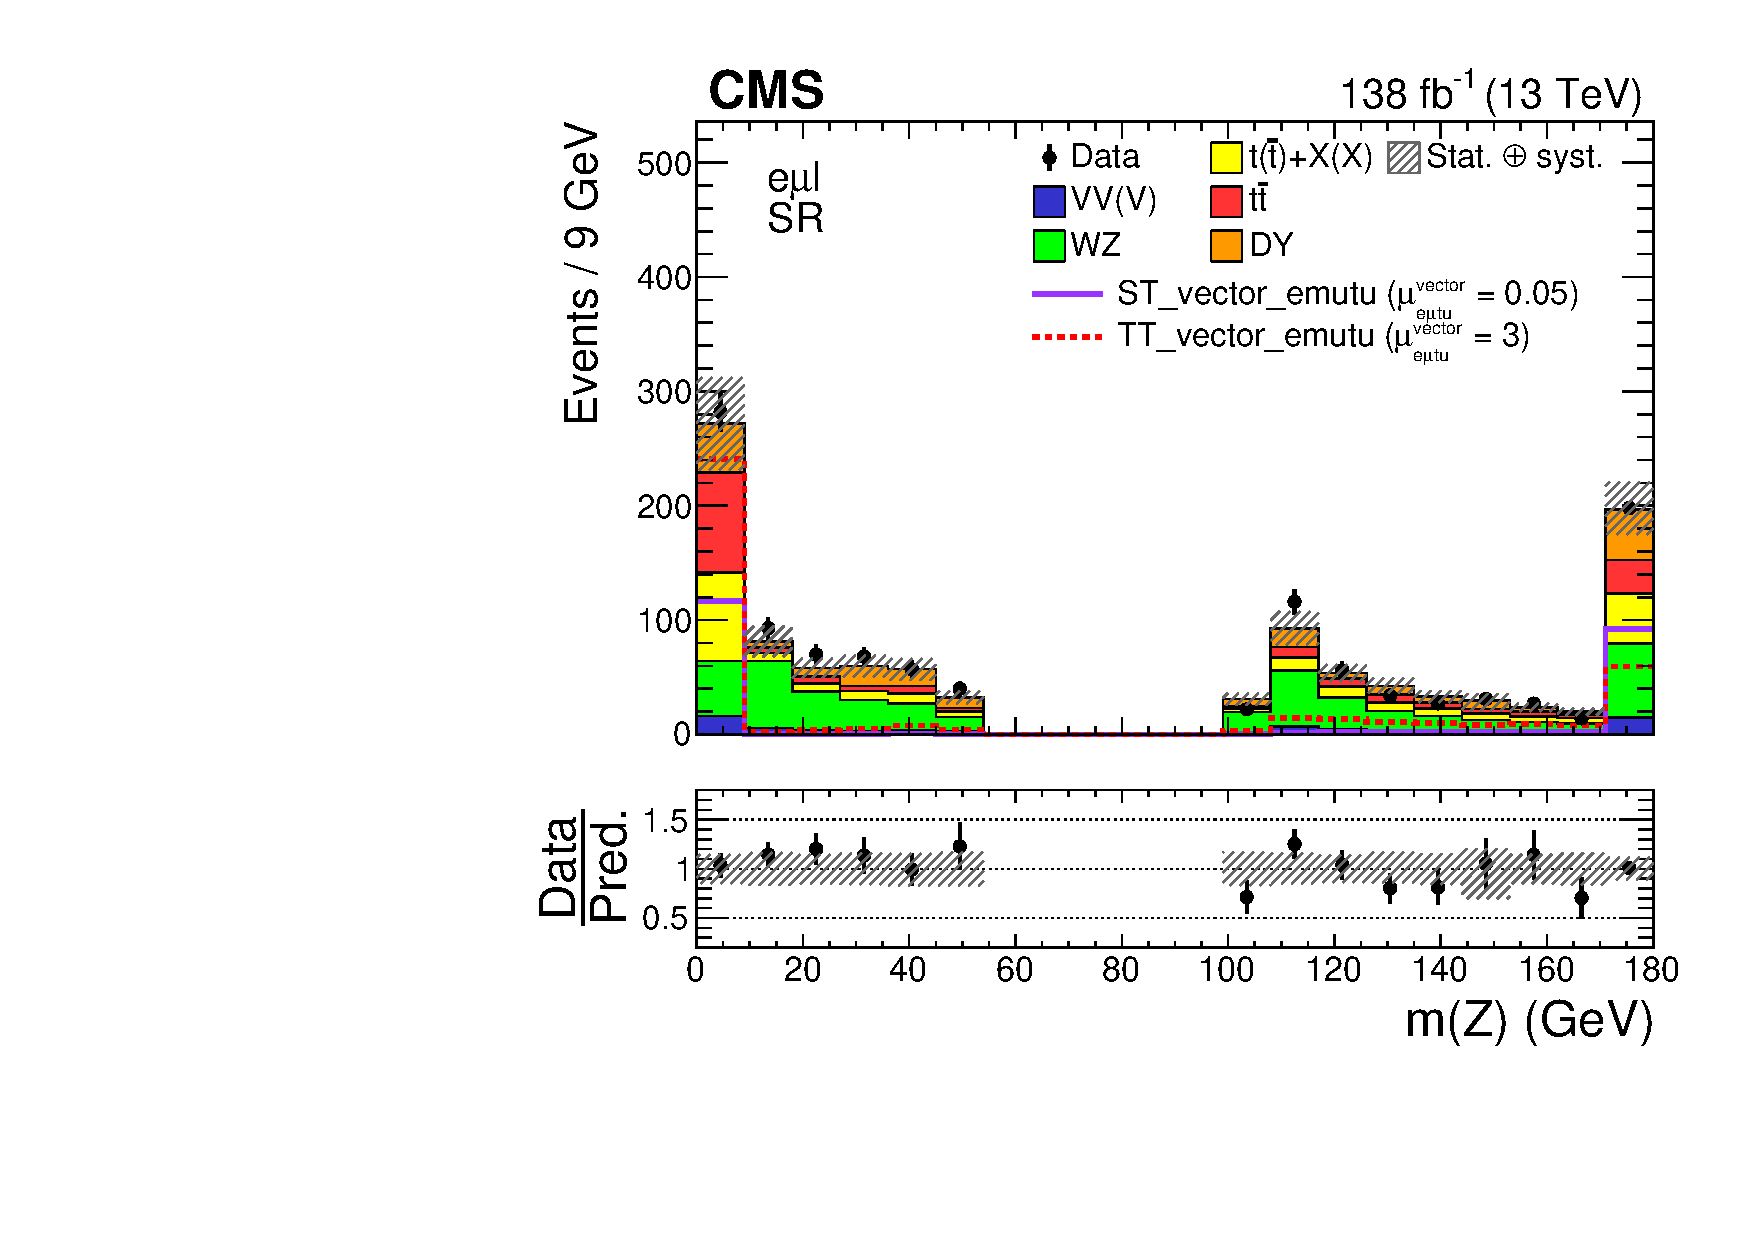
\includegraphics[width=0.45\textwidth]{figures/Part3/Selection/Zmass} \\
 \end{tabular}
 \caption{Distributions of different kinematic variables estimated in SR (full run II). Backgrounds are estimated using MC only. From left to right: invariant mass of the $e\mu$ pair, leading lepton $p_{T}$.}
 \label{fig:SR}
 \end{center}
\end{figure}

Using the invariant mass of the Opposite-Sign $e\mu$ pair, SR is further divided into two subsets to create ST and TT enriched regions:
\begin{itemize}
\item SR1, $M_{e\mu}<$150GeV: TT enriched.
\item SR2, $M_{e\mu}>$150GeV: ST enriched.
\end{itemize}
%%%%%%%%%%%%%%%%%%%%%%%%%%%%%%%%%%%%%%%%%%%%%%%%%%%%%%%%%%%%%
%%%%%%%%%%%%%%%%%%%%%%%%%%%%%%%%%%%%%%%%%%%%%%%%%%%%%%%%%%%%%
\section{Validation Region}
\label{sec:VR}

Events are required to pass trigger requirements listed in Table \ref{tab:triggers16}-\ref{tab:triggers18}. The leading lepton is required to have a $p_{T}>$38 GeV. The sum of the charges of the three selected leptons is required to be either 1 or -1. Selections applied to different regions are summarized in Table \ref{tab:region} and are illustrated in Figure \ref{fig:Event}. 
\begin{itemize}
\item Acronyms
\begin{itemize}
\item $C_i$: electric charge of the i-th lepton
\item OnZ: requiring the presence of at least one Opposite-Sign-Same-Flavor lepton pair with an invariant mass between 50 GeV and 106 GeV.
\item OffZ: veto events that pass OnZ
\item MET: missing transverse energy 
\item njet: number of jets that pass jet selection
\item nbjet: number of b-tag jets that pass jet selection 
\item SR: signal region
\item VR: validation region for data-driven method
\item WZ CR: WZ control region
\end{itemize}
\end{itemize}

\begin{table}[th]
\sffamily
\centering
\begin{tabular}{cccccccc}
\toprule
Channel         &Region & $|\Sigma_iC_i|$=1 & OnZ & OffZ & MET $>$ 20 GeV &njet$>=$1 &nbjet$<=$1\\ \midrule
\multirow{2}{*}{eee}     & VR & \checkmark & -       & -       & -       & -     & -   \\  
            & WZ VR &\checkmark & \checkmark   & -       & \checkmark   & \checkmark & \checkmark\\ \midrule
\multirow{3}{*}{e$\upmu\ell$}   & SR & \checkmark  & -       & \checkmark   & \checkmark   & \checkmark & \checkmark \\
            & Nonprompt VR & \checkmark  & \checkmark   & -       & -       & -     & -     \\
            & WZ VR & \checkmark & \checkmark   & -       & \checkmark   & \checkmark & \checkmark \\ \midrule
\multirow{2}{*}{$\upmu\upmu\upmu$} & Nonprompt VR & \checkmark   & -       & -       & -       & -     & -     \\  
            & WZ VR & \checkmark & -       & \checkmark   & \checkmark & \checkmark & \checkmark  \\ \bottomrule  
\end{tabular}
\caption{Summary of the cuts applied to different regions}
\label{tab:region}
\end{table}

\begin{figure}[tbh!]
 \begin{center}
 \begin{tabular}{c}
 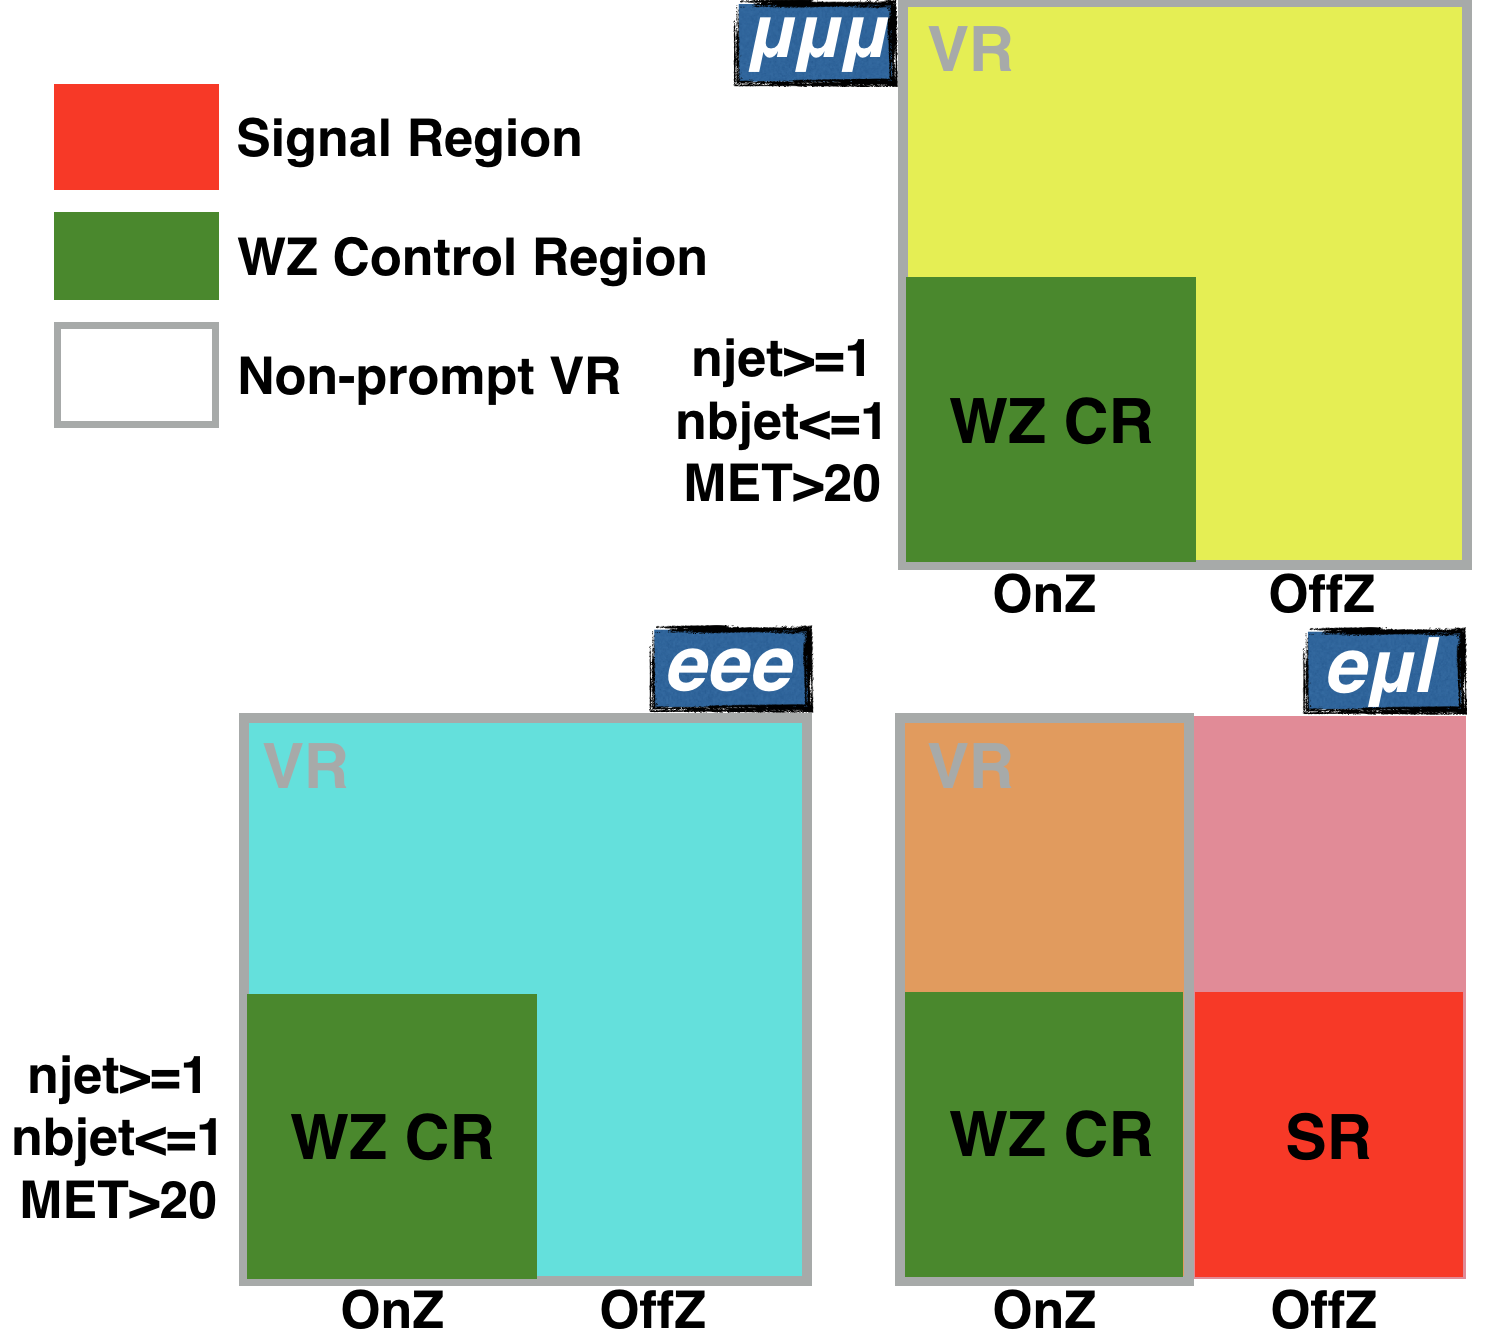
\includegraphics[width=0.8\textwidth]{figures/Part3/Selection/Event}
 \end{tabular}
 \caption{Illustration of event selections applied to different regions}
 \label{fig:Event}
 \end{center}
\end{figure}

There are two types of signal-depleted regions defined within eee/$\mu\mu\mu$ channel: validation region (VR) and WZ control region. The distinction between these two regions comes down to background compositions. It is expected that the VR has a significant fraction of non-prompt backgrounds while WZ production is responsible for most of the backgrounds in the WZ control region. Distributions of leading lepton $p_{T}$ and leading lepton $\eta$ in WZ control region can be found in Figure~\ref{fig:WZ_eee}-\ref{fig:WZ_mumumu}. Discussion about validation region can be found in \autoref{chap:Nonprompt}.

\begin{figure}[tbh!]
 \begin{center}
 \begin{tabular}{cc}
 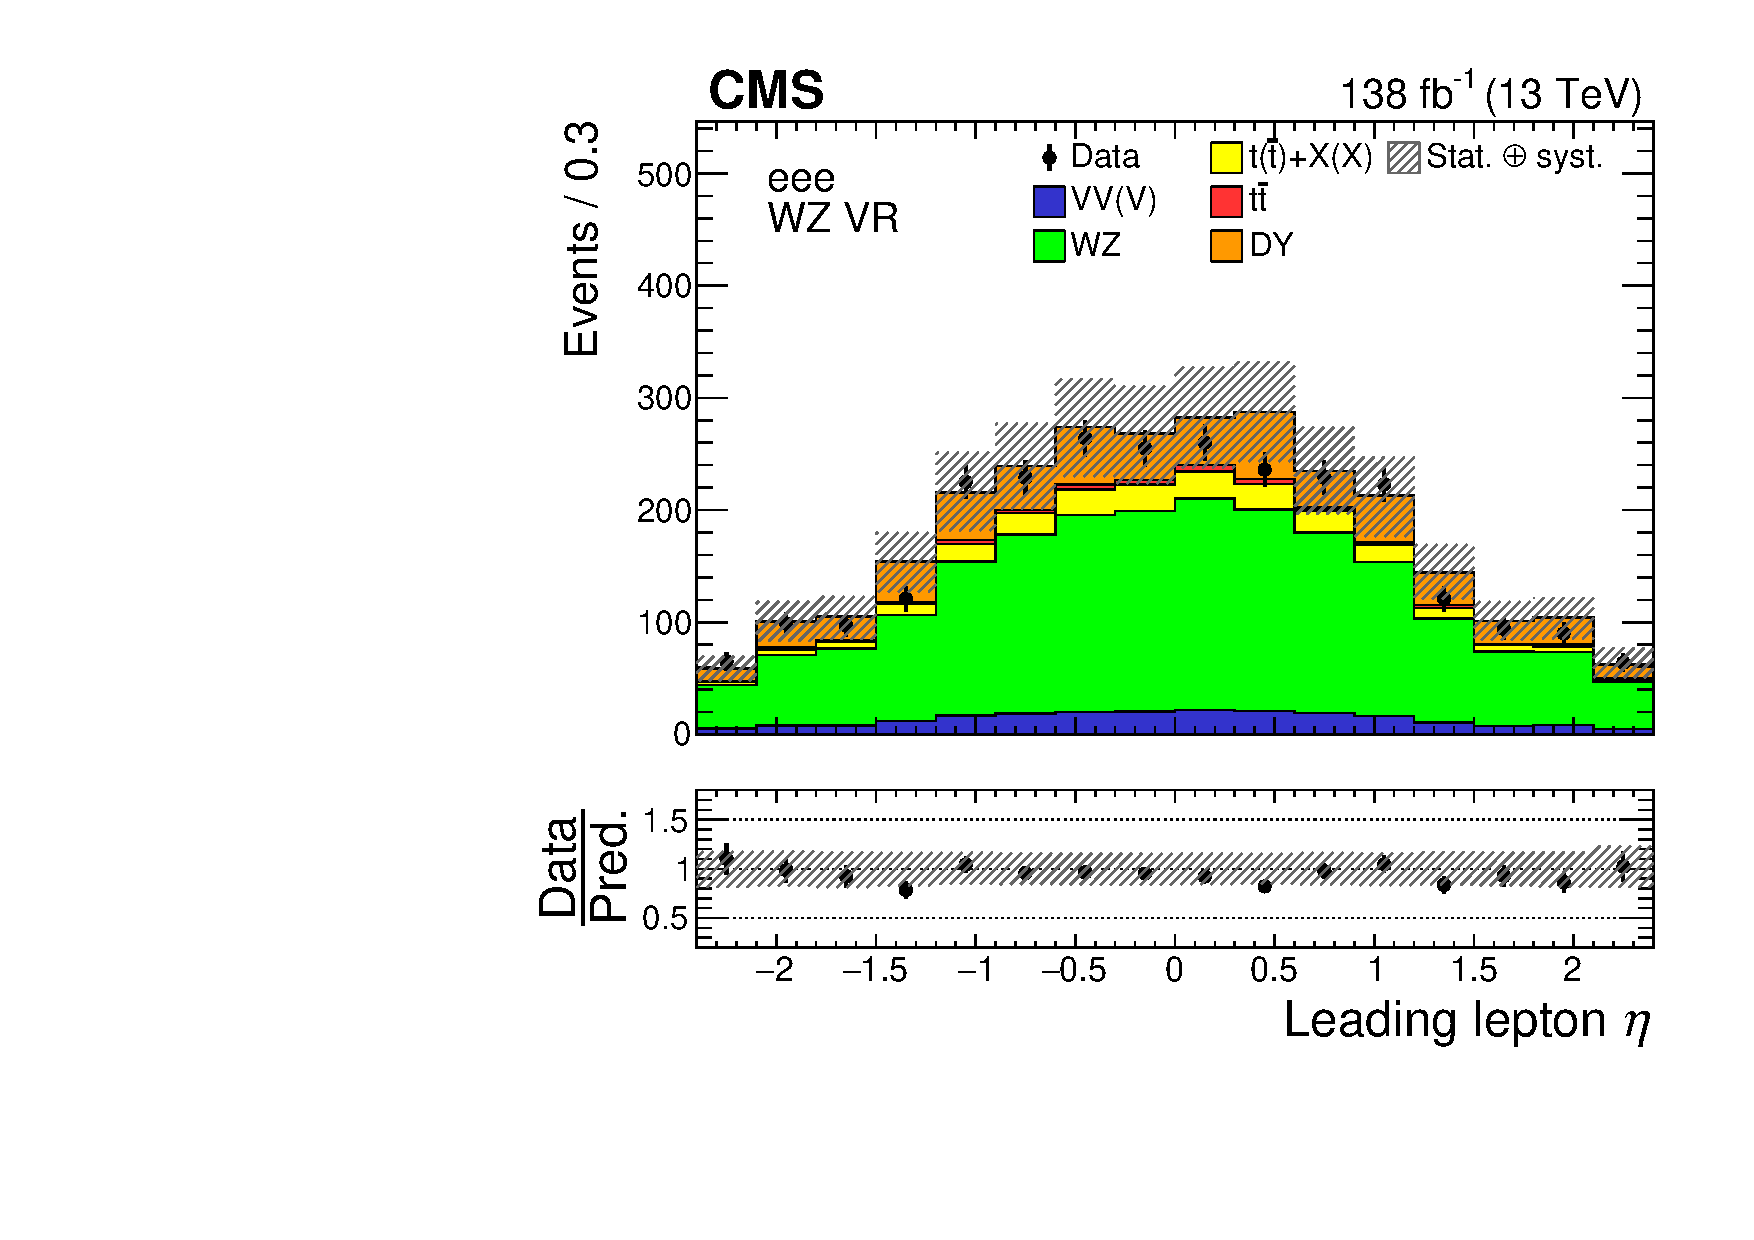
\includegraphics[width=0.45\textwidth]{figures/Part3/Selection/WZ/eee/lep1Eta}&
 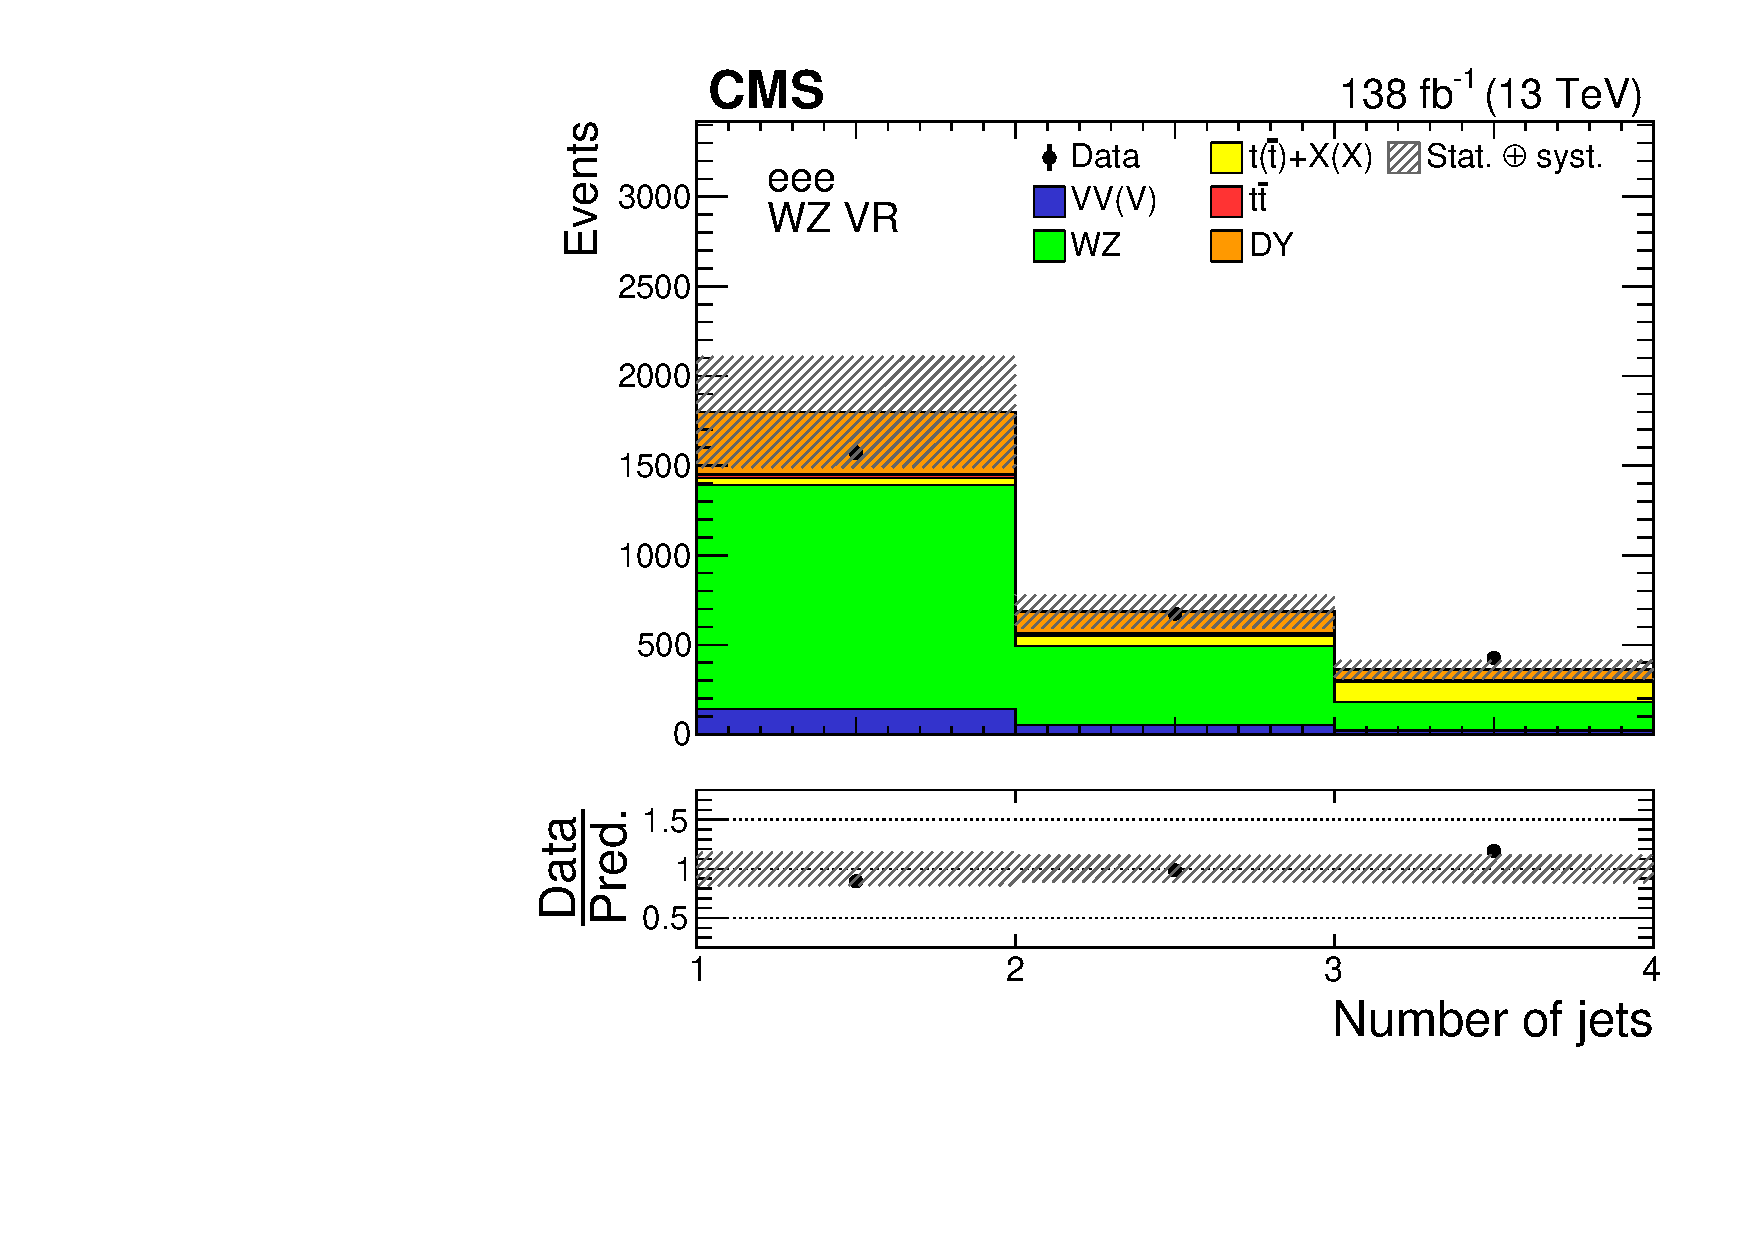
\includegraphics[width=0.45\textwidth]{figures/Part3/Selection/WZ/eee/njet} \\
 \end{tabular}
 \caption{Distributions of different kinematic variables estimated in WZ control region (full run II). Backgrounds are estimated using MC only. From left to right: leading lepton $\eta$, jet multiplicity.}
 \label{fig:WZ_eee}
 \end{center}
\end{figure}

\begin{figure}[tbh!]
 \begin{center}
 \begin{tabular}{cc}
 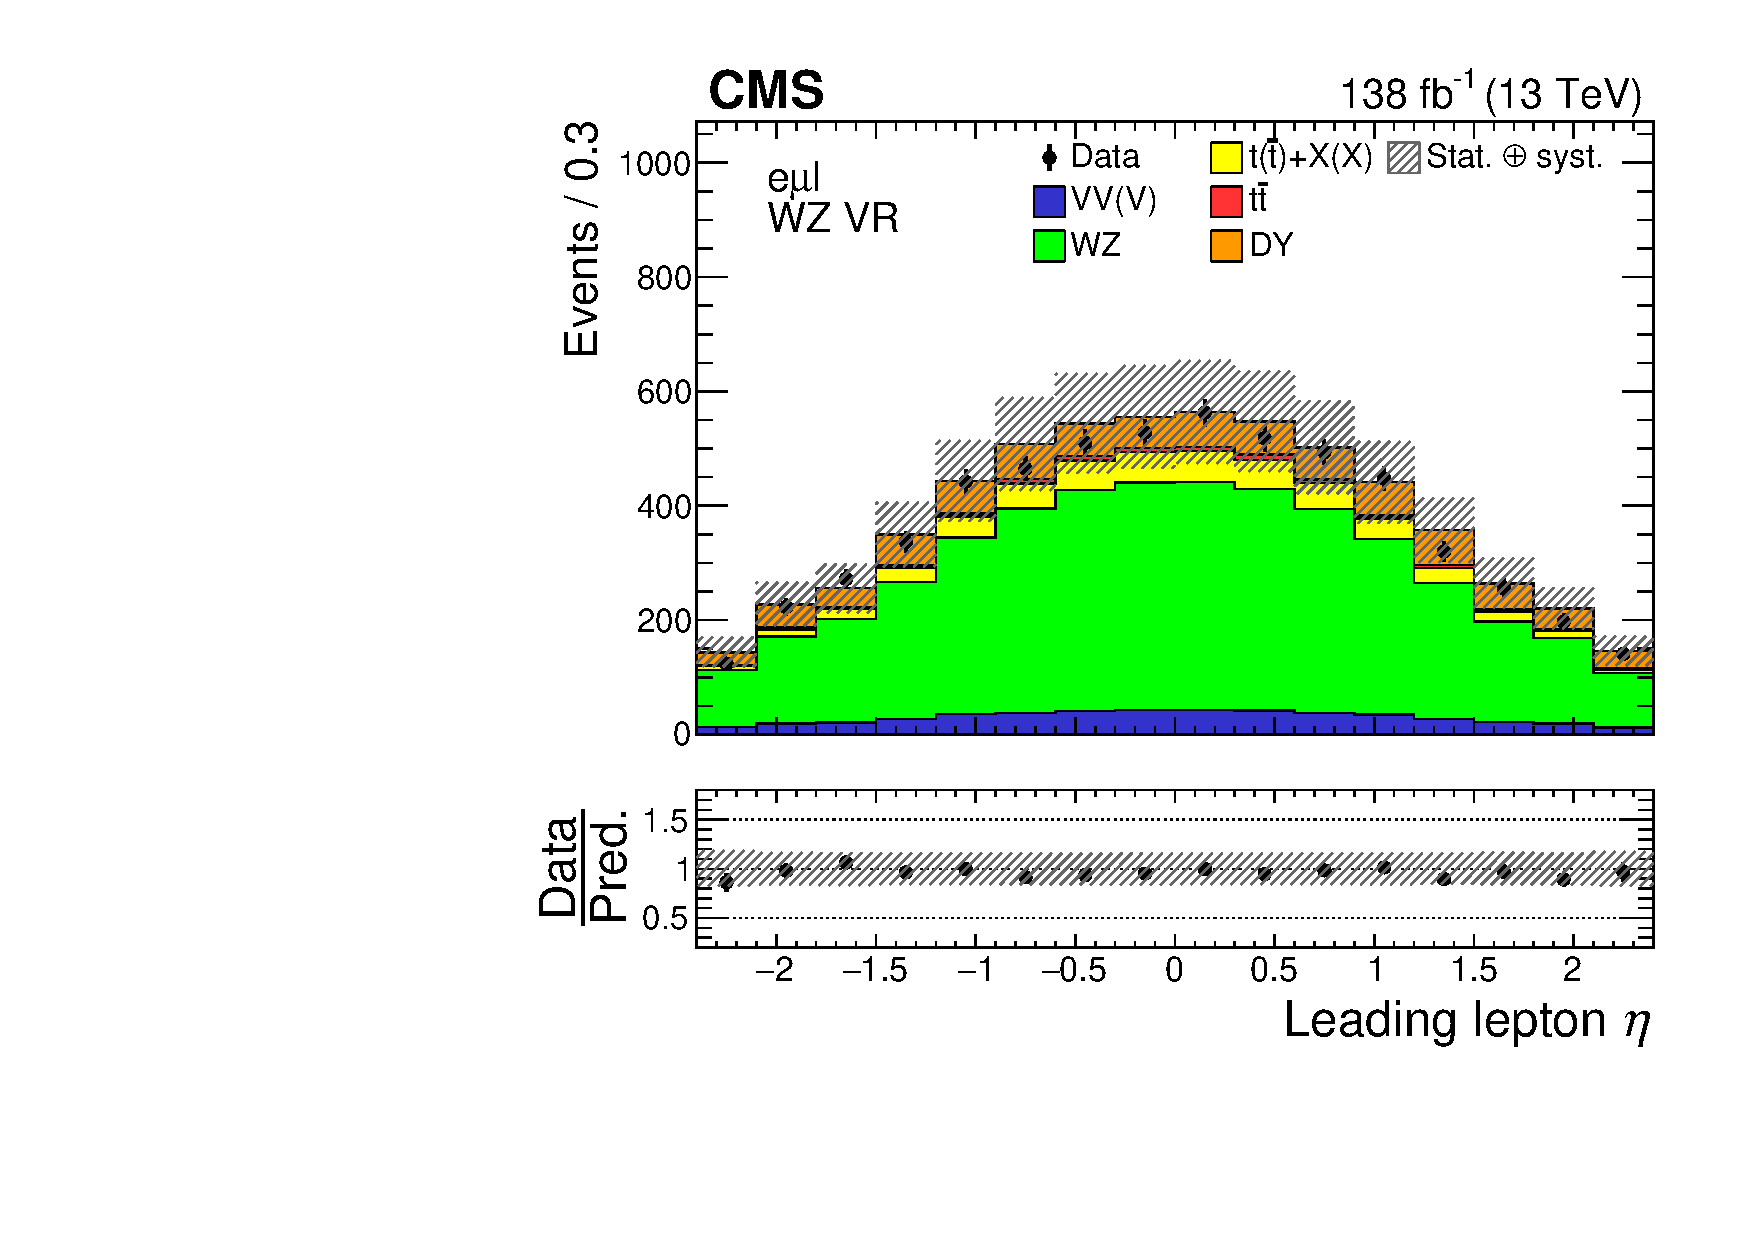
\includegraphics[width=0.45\textwidth]{figures/Part3/Selection/WZ/emul/lep1Eta}&
 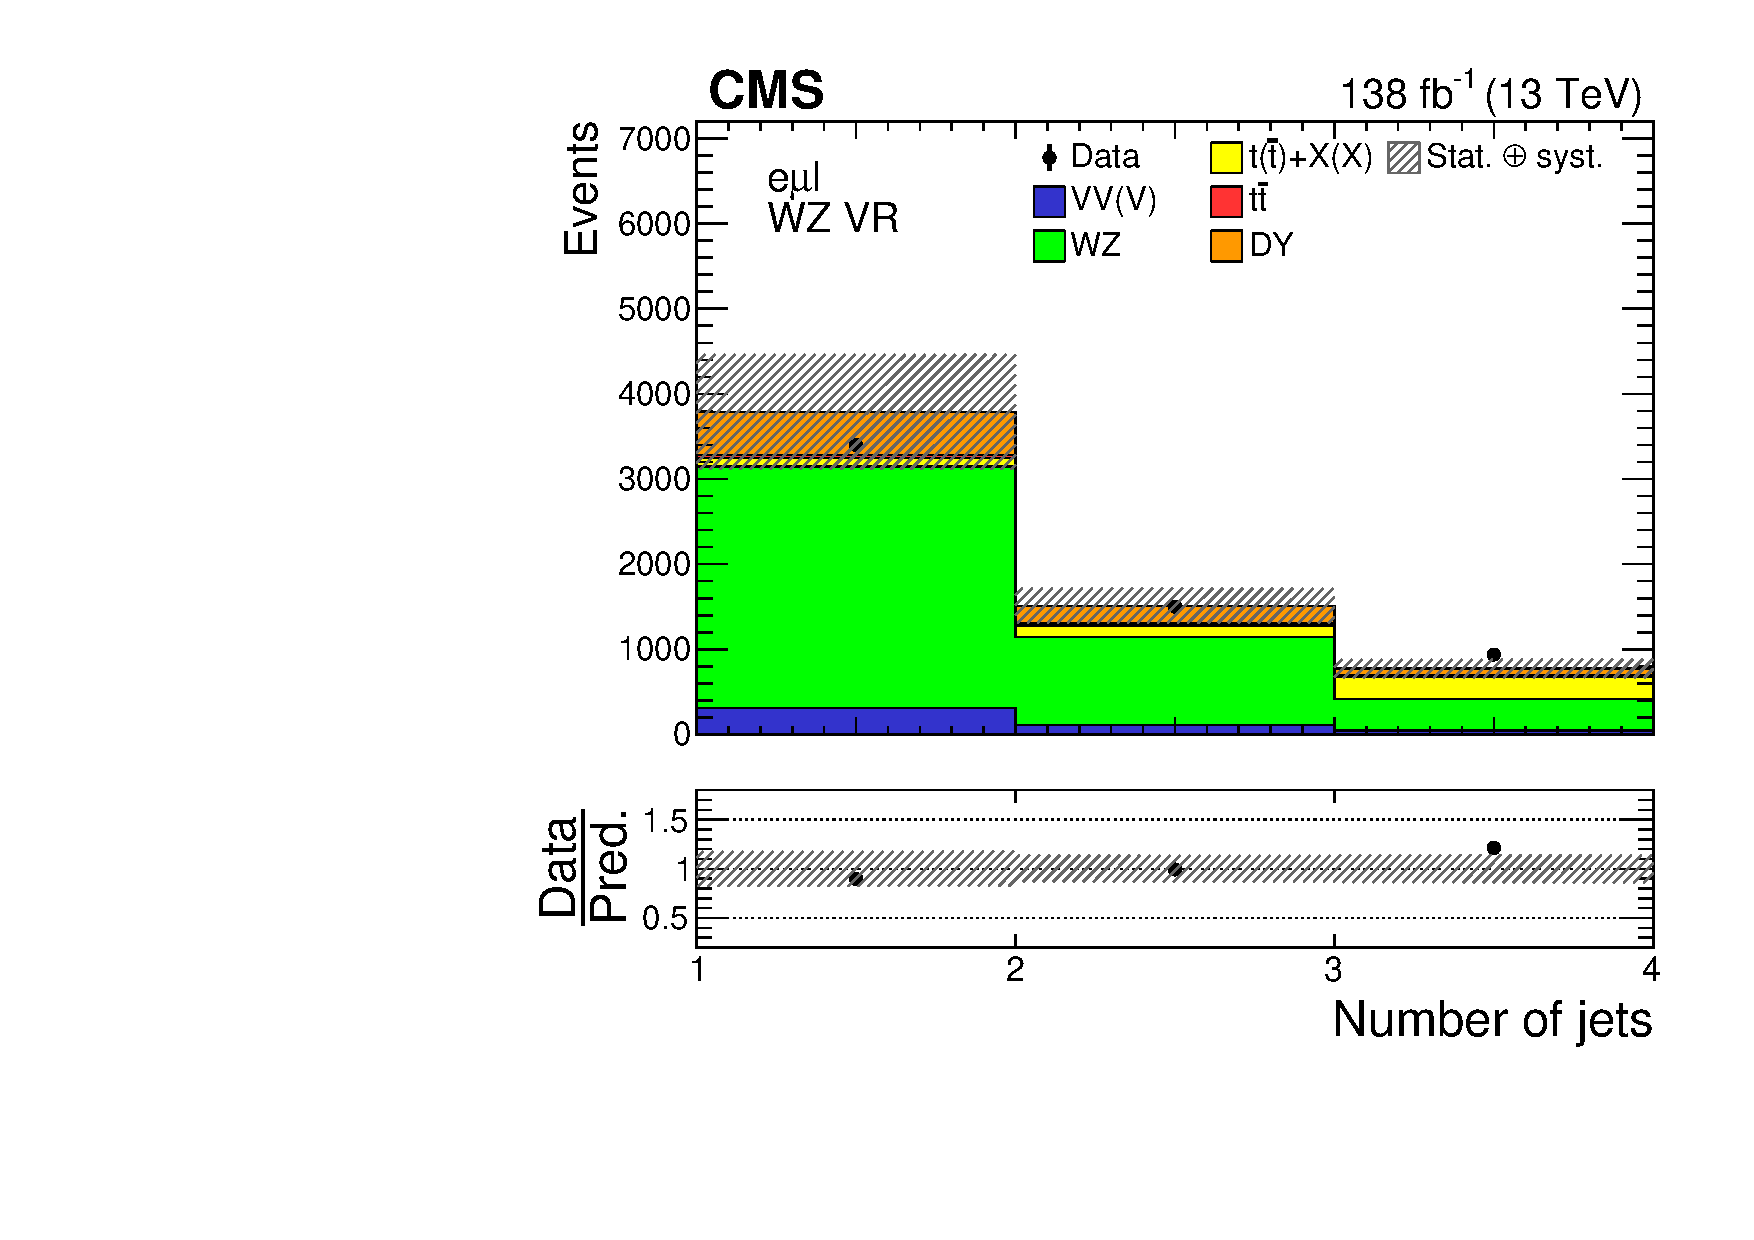
\includegraphics[width=0.45\textwidth]{figures/Part3/Selection/WZ/emul/njet} \\
 \end{tabular}
 \caption{Distributions of different kinematic variables estimated in WZ control region (full run II). Backgrounds are estimated using MC only. From left to right: leading lepton $\eta$, jet multiplicity.}
 \label{fig:WZ_emul}
 \end{center}
\end{figure}

\begin{figure}[tbh!]
 \begin{center}
 \begin{tabular}{cc}
 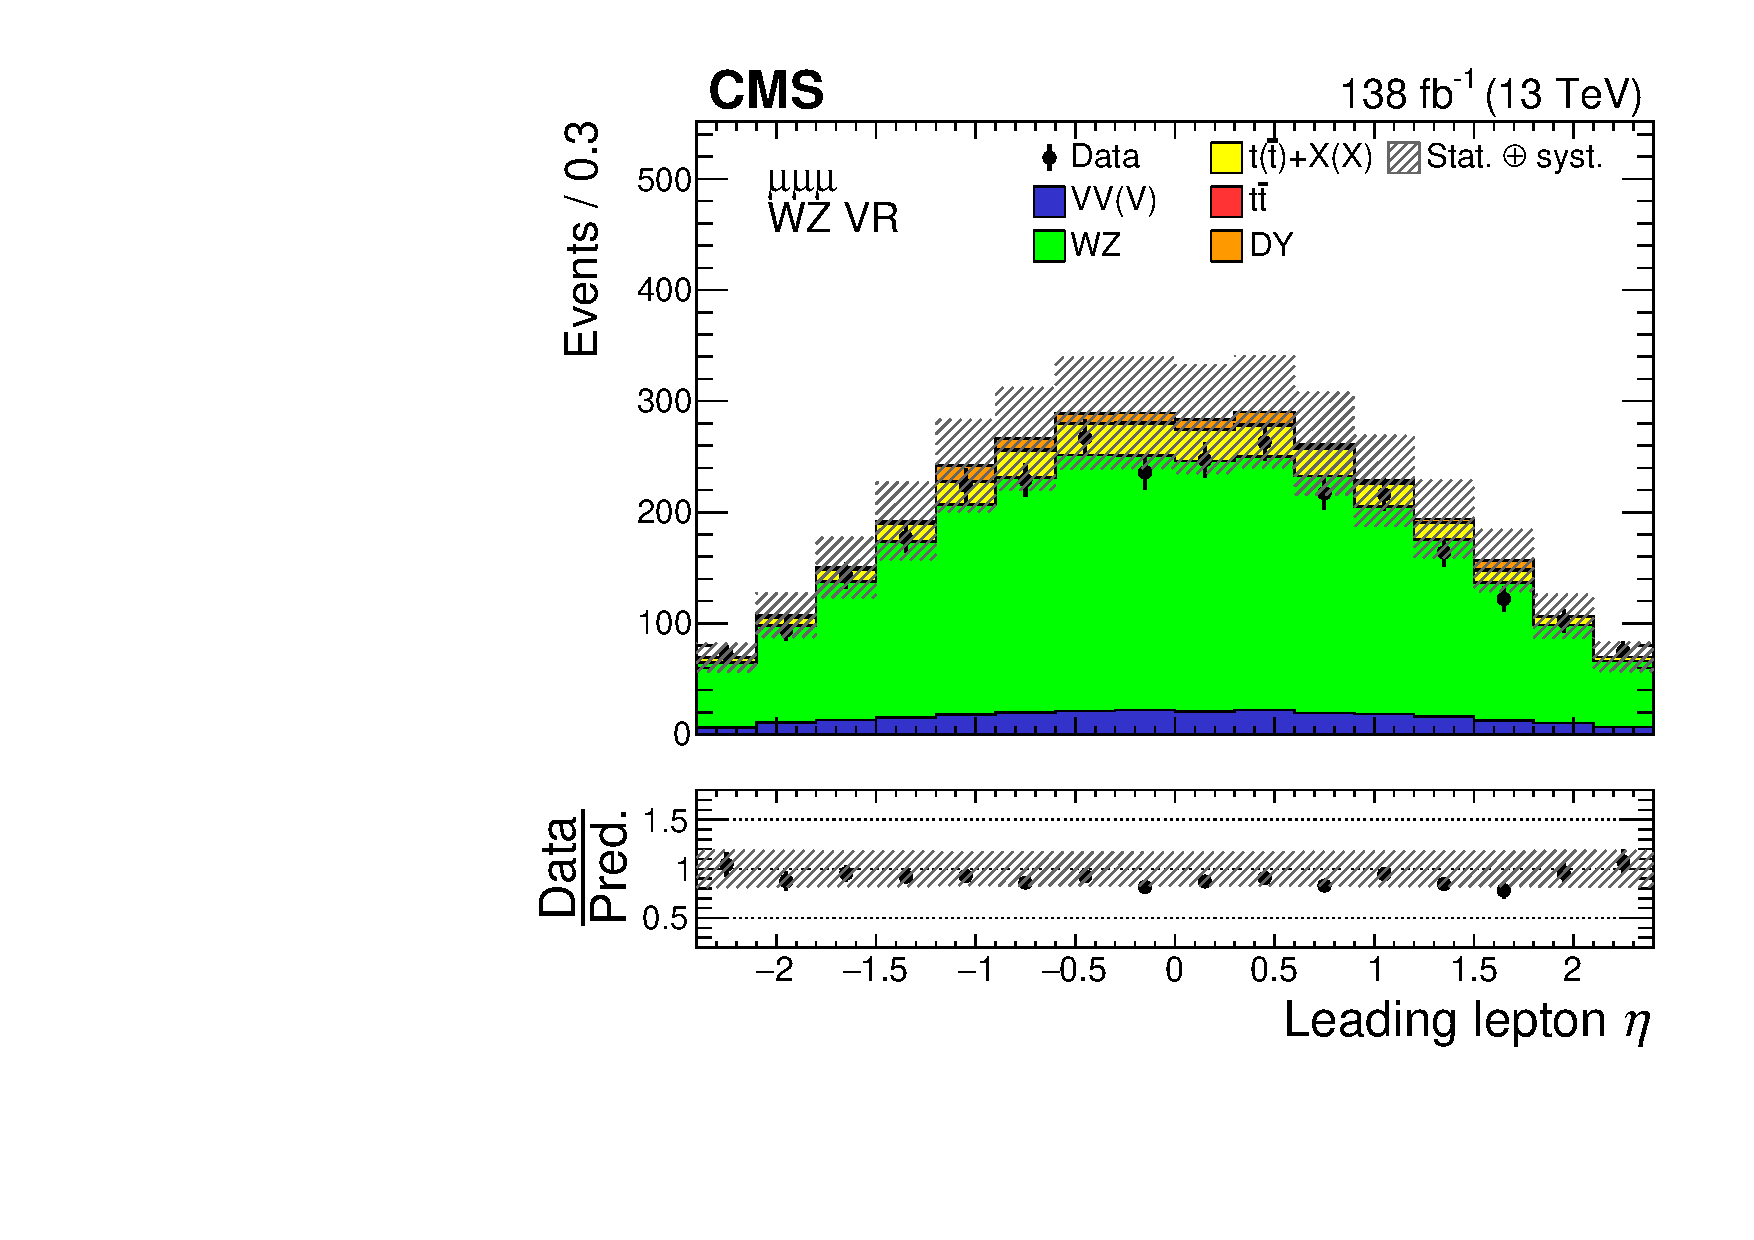
\includegraphics[width=0.45\textwidth]{figures/Part3/Selection/WZ/mumumu/lep1Eta}&
 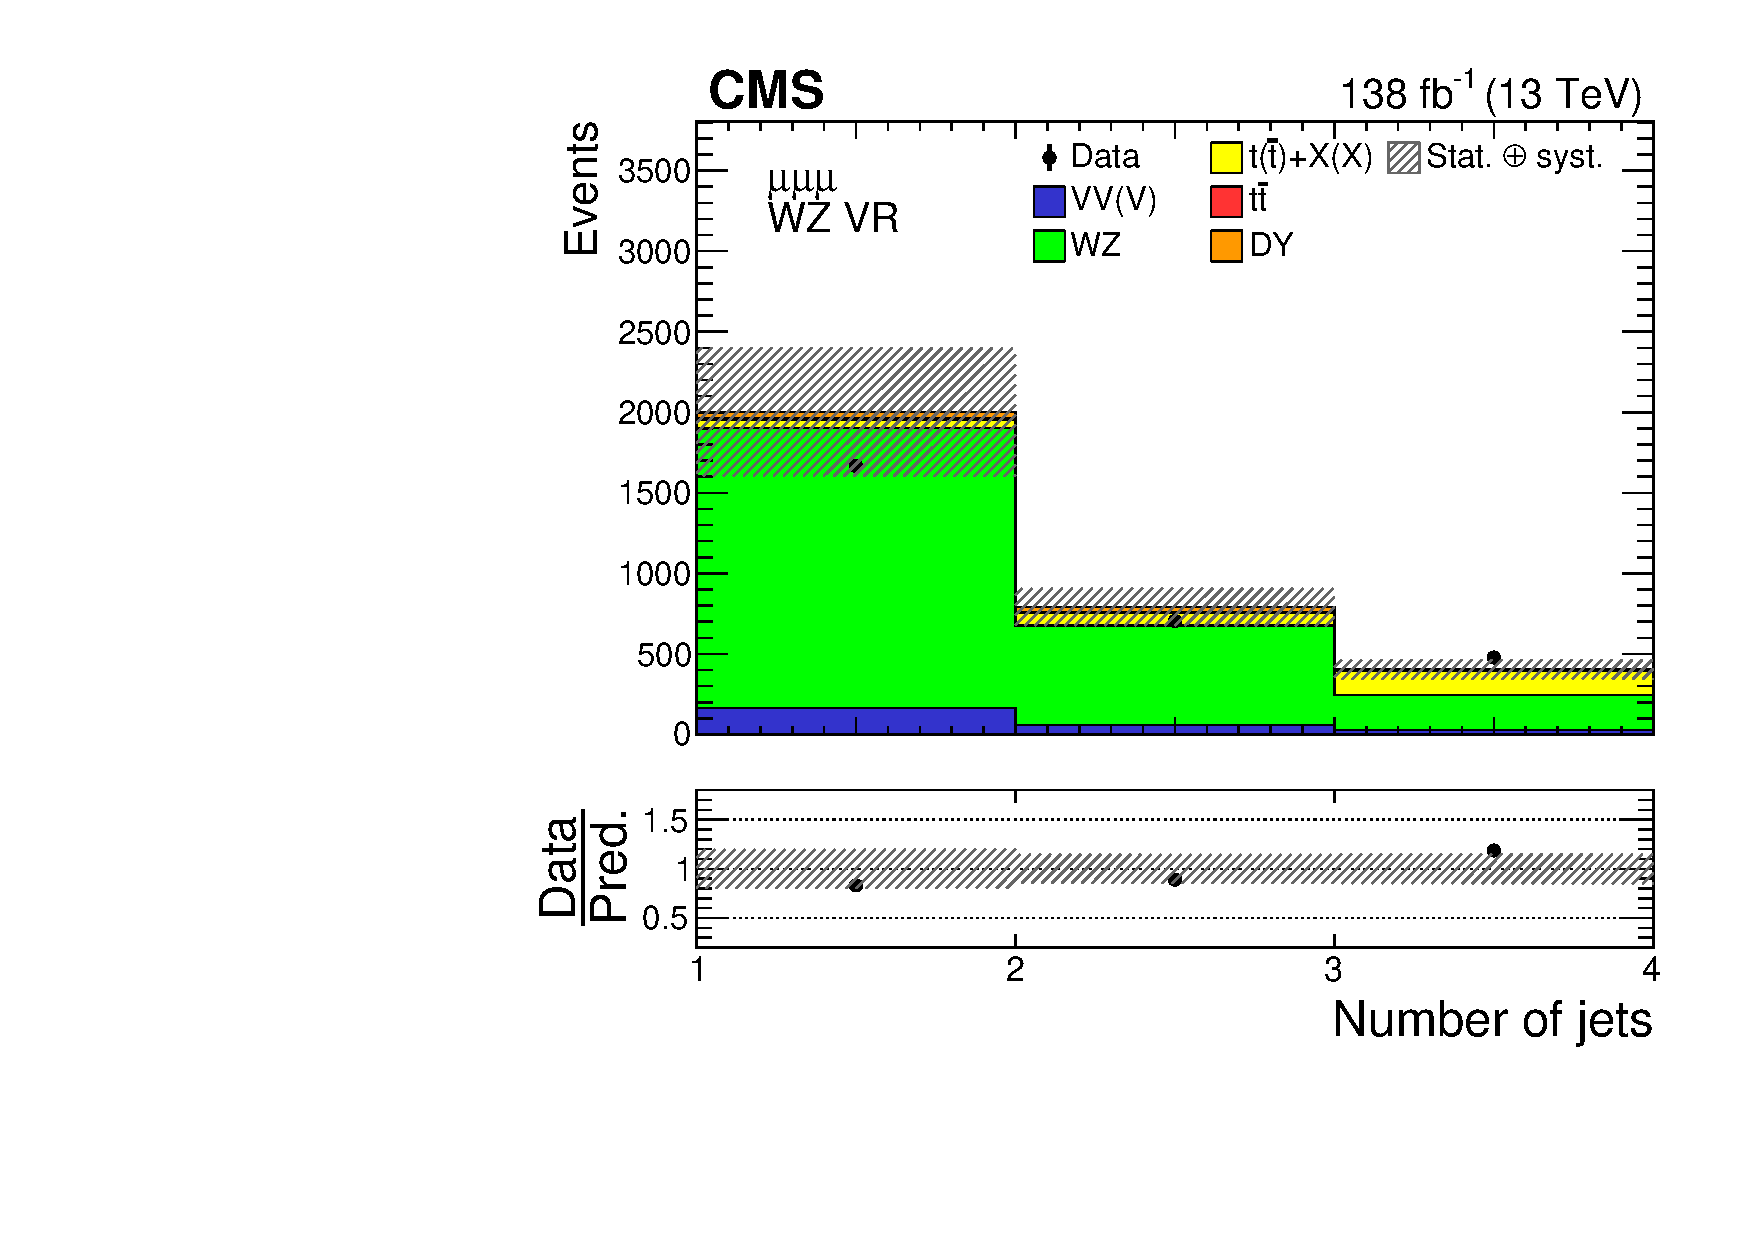
\includegraphics[width=0.45\textwidth]{figures/Part3/Selection/WZ/mumumu/njet} \\
 \end{tabular}
 \caption{Distributions of different kinematic variables estimated in WZ control region (full run II). Backgrounds are estimated using MC only. From left to right: leading lepton $\eta$, jet multiplicity.}
 \label{fig:WZ_mumumu}
 \end{center}
\end{figure}
%%%%%%%%%%%%%%%%%%%%%%%%%%%%%%%%%%%%%%%%%%%%%%%%%%%%%%%%%%%%%
%%%%%%%%%%%%%%%%%%%%%%%%%%%%%%%%%%%%%%%%%%%%%%%%%%%%%%%%%%%%%
\section{Kinematic Reconstruction}
\label{sec:Kin}
A kinematic reconstruction is performed in this channel. The OSOF lepton pair is assumed to be the product of cLFV interaction, while the third lepton (bachelor lepton) is assumed to be the product of the SM top-quark decay. Jet with the highest b-tagging score is assumed to originate from bottom-quark decay, therefore, it is combined with MET and the bachelor lepton to build the SM top-quark. 

\begin{itemize}
\item We take the x and y component of MET as measurements of neutrino $p_x$ and $p_y$. 
\item The z component of neutrino momentum is calculated by imposing the constraint that the invariant mass of the combined object (bachelor lepton+neutrino) must be equal to W boson mass.
\item If there is no real solution, we take the real part of the complex solution.
\item If there is more than one real solution, we chose the solution that is the closest to the $p_z$ of the bachelor lepton.
\end{itemize}

In events where there is more than one candidate of bachelor lepton, the lepton that gives a top mass that is the closest to the the SM top-quark mass is chosen as the bachelor lepton.

Once the bachelor lepton has been determined, the OSOF pair is combined with jets One-By-One to reconstruct LFV top candidates. Jet with the highest b-tagging score is excluded from this reconstruction since it is assumed to be from the decay of the SM top-quark. Out of all the LFV top candidates, the candidate that gives a top mass that is the closest to the the SM top-quark mass is chosen.

Kinematic reconstruction of heavy objects like top-quark is carried out using selected leptons, jets, and MET.
\begin{itemize}
\item \textbf{Z boson candidate}
\begin{itemize}
\item Z boson candidate is reconstructed by combining two Opposite-Sign-Same-Flavor leptons 
\item Whenever possible, Z candidate with an invariant mass that is closest to Z boson mass is chosen
\end{itemize}
\item \textbf{Standard model top-quark candidate }
\begin{itemize}
\item Standard model top-quark candidate is reconstructed by combining a jet, a lepton, and MET
\item Jet with the highest b-tagging score is always chosen
\item In $e\mu l$ channel, flavor-violating leptons are excluded from reconstruction 
\begin{itemize}
\item Whenever more than one lepton is available due to possible combinatorics of flavor-violating $e\mu$ pair, lepton that forms a top-quark candidate with an invariant mass that is closest to the top-quark mass is chosen 
\end{itemize}
\item In $eee$/$\mu\mu\mu$ channel, leptons that form Z candidate are excluded 
\item Lepton is combined with MET to reconstruct W candidate 
\begin{itemize}
\item Transverse component of the neutrino momentum is taken from MET
\item Neutrino $p_z$ is obtained by W mass constrain set on the lepton-neutrino system 
\end{itemize}
\end{itemize}
\item \textbf{Flavor-violating top-quark candidate }
\begin{itemize}
\item Flavor-violating top-quark candidate is reconstructed by combining a jet and an Opposite-Sign $e\mu$ lepton pair
\item Jet with the highest b-tagging score is excluded from reconstruction unless it fails b-tagging 
\item Whenever possible, the jet that forms a flavor-violating top-quark candidate with an invariant mass that is the closest to the top-quark mass is chosen
\item Lepton that forms the standard model top-quark candidate is excluded 
\end{itemize}
\item \textbf{The first b-jet+lepton system }
\begin{itemize}
\item Jet with the highest b-tagging score is always chosen 
\item All three leptons can form this system with the chosen jet 
\begin{itemize}
\item Lepton that forms a jet-lepton system with the lowest invariant mass is chosen 
\end{itemize}
\end{itemize}
\item \textbf{The second b-jet+lepton system}
\begin{itemize}
\item Jet with the highest b-tagging score is excluded unless it passes b-tagging 
\item Whenever possible (after the previous step), jet with the highest b-tagging score is chosen 
\item Lepton that forms the first jet-lepton system is excluded 
\item Leptons that have the same sign as the lepton that forms the first jet-lepton system is excluded 
\item Whenever possible, lepton that forms a jet-lepton system with the lowest invariant mass is chosen 
\end{itemize}
\end{itemize}